\documentclass[10pt]{extarticle}
\usepackage[sfdefault]{FiraSans}
\usepackage[T1]{fontenc}
\usepackage[utf8]{inputenc}
\usepackage{adjustbox}
\usepackage{algorithm}
\usepackage{algorithmic}
\usepackage{amsfonts}
\usepackage{amsmath}
\usepackage{amssymb}
\usepackage[style=apa]{biblatex}
\addbibresource{references.bib}
\usepackage{booktabs}
\usepackage{breqn}
\usepackage{enumitem}
\usepackage{float}
\usepackage{geometry}
\usepackage{graphicx}
\usepackage{hyperref}
\usepackage{lipsum}
\usepackage{longtable}
\usepackage{multirow}
\usepackage{pdfpages}
\usepackage{pgfgantt}
\usepackage{setspace}
\usepackage{subcaption}
\usepackage{tabularx}
\usepackage{tikz}
\usepackage{xcolor}

\DeclareLanguageMapping{english}{english-apa}

\geometry{letterpaper, left=1in, right=1in, top=1in, bottom=1in,}

\definecolor{primary}{RGB}{0,120,215}
\definecolor{secondary}{RGB}{255,87,34}
\definecolor{background}{RGB}{245,245,245}
\definecolor{blue}{RGB}{0,62,126}

\pagecolor{background}

\hypersetup{colorlinks=true, linkcolor=primary, filecolor=secondary, urlcolor=primary, citecolor=black}

\AtBeginBibliography{\hypersetup{urlcolor=black}}

\setstretch{1.15}

\setlength{\bibhang}{0.5in}
\setlength\bibitemsep{1.5\itemsep}

\setlength{\parindent}{0pt}
\setlength{\parskip}{1em}

\nocite{*}

\begin{document}

\newcommand{\mytitlepage}[2]{
    \thispagestyle{empty}

    \begin{tikzpicture}[remember picture, overlay]
        \node [inner sep=0pt] at (current page.center) {#1}; { \node [ anchor=center, inner sep=1.25cm, rectangle, fill=blue!70!white, fill opacity=0, text opacity=1, minimum height=0.2\paperheight, minimum width=\paperwidth, text width=0.8\paperwidth, font=\fontfamily{pnc}\selectfont ] at (current page.center) {#2}; } \node [anchor=south east, outer sep=3pt] at (current page.south east) {
\includegraphics[width=0.33\paperwidth]{logo.png}};
    \end{tikzpicture}

    \newpage
}

{ \mytitlepage{\includegraphics[width=\paperwidth]{background.png}}
    {
        \centering
        \fontfamily{phv}
        \vspace{-200pt} % move title up
        { \Huge
            \bfseries

            \begin{center}
                Next-Generation Health Monitoring: \\
                A Real-Time Approach to Fitness Tracking
            \end{center}

            \par
        }
        \vspace{8pt}
        { \Large
            \bfseries

            Final Report

            \par
        }
        \vspace{24pt}
        {
            \begin{center}
                \begin{tabular*} {\textwidth}{@{\extracolsep{\fill}}c c c}
                    {\LARGE Jonathan Agustin} & {\LARGE Alec Anderson} & {\LARGE Brandon Smith}
                \end{tabular*}
            \end{center}
        }
    }
}

\pagenumbering{arabic}

\begin{center}
    {\LARGE \textbf{Next-Generation Health Monitoring}} \\
    {\large \textbf{A Real-Time Approach to Fitness Tracking}}
\end{center}

\section{Abstract}

We present a novel approach to sleep quality analysis by integrating Long Short-Term Memory (LSTM) networks with traditional machine learning techniques, utilizing data harvested from Fitbit devices. This study, situated at the confluence of computational health informatics and machine learning, aims to enhance the predictive accuracy and interpretability of sleep quality metrics derived from wearable technology. Through meticulous preprocessing, exploratory data analysis, and innovative feature engineering, we construct models that not only predict sleep quality with high fidelity but also offer insights into the underlying patterns of sleep behavior. Our methodology exemplifies the synergy between deep learning and traditional statistical models, showcasing their combined potential in extracting nuanced insights from complex, time-series health data. This research contributes to the burgeoning field of personalized health monitoring, offering a scalable framework for leveraging IoT data in health informatics.

\textbf{Keywords:} Sleep Quality, LSTM, Machine Learning, Fitbit Data, Health Informatics.

\section{Introduction}

\subsection{Problem Motivation}

The significance of sleep in maintaining and enhancing overall health cannot be overstated. Quality sleep is intricately linked to a myriad of health outcomes, influencing everything from cognitive performance and mood regulation to metabolic health and immune function. Despite its critical role, the monitoring and analysis of sleep quality often do not receive the attention they deserve in personal health management and clinical settings. This oversight can be attributed to the challenges inherent in accurately measuring and interpreting sleep data, which traditionally required intrusive and expensive polysomnography in sleep laboratories.

The proliferation of Internet of Things (IoT) devices, particularly wearable technology like Fitbit, has revolutionized the landscape of sleep monitoring. These devices offer a non-invasive, cost-effective means of collecting detailed sleep data, including metrics such as sleep duration, restlessness, and sleep stages. This wealth of data opens up new avenues for research and application, particularly in the domain of machine learning, where sophisticated algorithms can be trained to uncover patterns and predict sleep quality with unprecedented precision.

However, the intersection of Long Short-Term Memory (LSTM) networks—a class of deep learning models adept at handling time-series data—and traditional machine learning techniques in the context of sleep data analysis remains relatively unexplored. This gap in research is notable, given the complementary strengths of these approaches. LSTM networks are particularly well-suited to modeling the temporal dependencies inherent in sleep data, while traditional machine learning techniques offer robust tools for feature extraction and interpretation.

The sparse exploration of this intersection represents a missed opportunity for advancing sleep science and developing personalized sleep monitoring solutions. By harnessing the predictive power of LSTM networks alongside the interpretative capabilities of traditional machine learning models, researchers and practitioners can gain deeper insights into sleep patterns, identify determinants of sleep quality, and tailor interventions to improve sleep health. This project is motivated by the potential of these combined methodologies to unlock new understandings of sleep and offer actionable insights that can enhance individual and population health.

\subsection{Research Gap}

The advent of wearable technology has ushered in an era of unprecedented data collection capabilities, particularly in the realm of sleep monitoring. Devices such as Fitbit offer detailed insights into various sleep metrics, including duration, restlessness, and sleep stages, providing a rich dataset for analysis. However, the potential of this data remains largely untapped due to a notable research gap: the integration of Long Short-Term Memory (LSTM) networks with traditional machine learning (ML) techniques for the predictive analysis of sleep quality.

LSTM networks, a subset of deep learning models, are renowned for their ability to process sequential data, making them ideally suited for analyzing the time-series data generated by wearable devices. Traditional ML techniques, on the other hand, excel in feature extraction and interpretation, providing valuable insights into the factors influencing sleep quality. Despite the complementary strengths of these methodologies, their combined application in the context of sleep data analysis is scarce. This oversight is particularly glaring given the complex, multifaceted nature of sleep, which encompasses various dimensions and temporal patterns that could be more effectively modeled through a hybrid analytical approach.

The limited exploration of this synergistic approach represents a significant research gap with profound implications for the field of sleep science and personalized health monitoring. By integrating the predictive power of LSTM networks with the interpretative capabilities of traditional ML models, researchers can unlock deeper insights into sleep patterns, identify key determinants of sleep quality, and develop more accurate, personalized sleep monitoring solutions. Such advancements could revolutionize our understanding of sleep and its impact on health, paving the way for targeted interventions and improved health outcomes.

Moreover, the research gap underscores a broader challenge in health informatics: the need for interdisciplinary approaches that leverage the strengths of diverse analytical techniques. Bridging this gap requires not only technical expertise in machine learning and data science but also a deep understanding of sleep physiology and the factors influencing sleep quality. Addressing this research gap, therefore, presents an opportunity to advance the field of digital health, contributing to the development of innovative tools and strategies for enhancing sleep quality and, by extension, overall well-being.

The integration of LSTM and traditional ML techniques for the analysis of sleep data from wearables represents a promising yet underexplored avenue of research. Closing this gap holds the potential to significantly advance personalized health monitoring and intervention, offering new insights and approaches for improving sleep quality and health outcomes.

\subsection{Project Contributions}

Our project leverages LSTM for its time-series prediction strengths and traditional ML for feature categorization, offering a novel approach to sleep quality prediction using IoT data. This interdisciplinary effort aims to enhance personalized health monitoring and contribute to the digital health landscape.

\section{Dataset and Preprocessing}

\subsection{Dataset Description}

The dataset employed in this study is derived from Fitbit devices, a popular brand of wearable technology that tracks various health-related metrics, including physical activity, heart rate, and sleep patterns. Specifically, our focus is on the sleep data collected by these devices, which provides a comprehensive overview of users' sleep behavior over an extended period. The dataset encompasses several thousand individual records, each corresponding to a single night's sleep for a given user. This wealth of data presents a unique opportunity to delve into the intricacies of sleep patterns and their implications for overall health and well-being.

Key features included in the dataset are as follows:

- \textbf{Timestamp:} The date and time when the sleep record was initiated, providing a temporal context for each entry.
- \textbf{Sleep Duration:} The total amount of time spent asleep during the night, measured in minutes. This metric is crucial for assessing whether individuals are meeting recommended sleep duration guidelines.
- \textbf{Restlessness:} A measure of movement during sleep, quantified as the percentage of time spent restless. High levels of restlessness may indicate disturbed sleep, potentially impacting sleep quality.
- \textbf{Sleep Stages:} The distribution of time spent in various sleep stages, including light sleep, deep sleep, and REM (Rapid Eye Movement) sleep. Understanding the proportion of time spent in each stage can offer insights into sleep architecture and quality.
- \textbf{Overall Sleep Score:} A composite metric calculated by Fitbit, summarizing the quality of sleep on a scale from 0 to 100. The sleep score is derived from a combination of factors, including sleep duration, restlessness, and time spent in different sleep stages.

The dataset's granularity and breadth enable a multifaceted analysis of sleep patterns, facilitating the exploration of correlations between sleep metrics and the identification of predictors of sleep quality. By leveraging this dataset, our project aims to develop predictive models that can accurately forecast sleep quality based on a range of sleep-related variables. Such models hold the potential to inform personalized sleep interventions, contributing to improved sleep hygiene and, by extension, enhanced health outcomes.

In preparing the dataset for analysis, we undertake a series of preprocessing steps to ensure data quality and compatibility with machine learning algorithms. These steps include handling missing values, encoding categorical variables, and standardizing numerical features. Through careful preprocessing and exploratory data analysis, we lay the groundwork for the application of advanced machine learning techniques, including Long Short-Term Memory (LSTM) networks and traditional classifiers, to uncover patterns and insights within the sleep data.

\subsection{Preprocessing}

Our preprocessing pipeline includes handling missing values with forward fill, encoding categorical variables, and standardizing features to prepare the dataset for machine learning analysis.

\section{Exploratory Data Analysis (EDA)}

\subsection{Descriptive Statistics}

Descriptive statistics serve as the foundation of our exploratory data analysis, offering a preliminary glimpse into the structure and characteristics of the sleep data collected from Fitbit devices. By examining measures of central tendency (mean, median) and dispersion (standard deviation, interquartile range), we gain valuable insights into the typical sleep behaviors and variability within our dataset. This section outlines our approach to analyzing key variables, specifically focusing on overall sleep score and restlessness, which are critical to assessing sleep quality.

\subsubsection{Overall Sleep Score}

The overall sleep score is a composite metric calculated by Fitbit, summarizing the quality of sleep on a scale from 0 to 100. Higher scores indicate better sleep quality, incorporating factors such as sleep duration, restlessness, and time spent in various sleep stages. Descriptive statistics for the overall sleep score reveal the average sleep quality experienced by participants and the range of sleep quality within the dataset.

- \textbf{Mean Sleep Score:} The mean provides an indication of the average sleep quality across all participants. A higher mean score suggests that, on average, participants experience good sleep quality.
- \textbf{Median Sleep Score:} The median offers insight into the central tendency of sleep quality, minimizing the impact of outliers. It represents the middle value when all sleep scores are arranged in ascending order.
- \textbf{Standard Deviation:} This measure indicates the variability of sleep scores around the mean. A larger standard deviation suggests a wider range of sleep quality experiences among participants.
- \textbf{Interquartile Range (IQR):} The IQR, calculated as the difference between the 75th and 25th percentiles, provides a measure of the middle 50\% of sleep scores. It helps identify the spread of the central half of the data.

\subsubsection{Restlessness}

Restlessness during sleep, quantified as the percentage of time spent restless, is a crucial indicator of sleep disturbance. Analyzing the descriptive statistics for restlessness can uncover patterns of sleep disruption among participants.

- \textbf{Mean Restlessness:} The average percentage of time spent restless during sleep. A lower mean suggests that participants generally experience less disruption during sleep.
- \textbf{Median Restlessness:} The median restlessness percentage, offering a robust measure of central tendency unaffected by extreme values.
- \textbf{Standard Deviation:} Reflects the variability in restlessness percentages across the dataset. A higher standard deviation indicates a greater diversity in sleep disruption experiences.
- \textbf{Interquartile Range (IQR):} Highlights the spread of the middle 50\% of restlessness data, providing insights into the typical range of sleep disruption.

By examining these descriptive statistics, we establish a baseline understanding of sleep quality and restlessness within our dataset. This analysis not only sheds light on the general sleep patterns observed but also identifies areas for deeper investigation, such as the factors contributing to high restlessness or the characteristics of individuals with exceptionally high or low sleep scores. These insights guide the subsequent phases of our analysis, including feature engineering and model development, ultimately aiming to predict sleep quality with greater accuracy and uncover strategies for improving sleep health.

\subsection{Visualizations}

In the realm of sleep quality analysis, visualizations play a pivotal role in unraveling the intricate patterns and distributions inherent in sleep-related metrics. Our study employs a suite of visualization techniques, including histograms, line plots, and correlation heatmaps, to dissect the multifaceted nature of sleep data derived from Fitbit devices. These visual tools not only facilitate a deeper understanding of the dataset at hand but also lay the groundwork for more informed feature engineering and model development processes.

\subsubsection{Histograms and Distribution Analysis}

Histograms serve as our primary tool for exploring the distribution of key sleep metrics, such as overall sleep score and restlessness. By plotting the frequency of occurrences for different ranges of these metrics, we gain valuable insights into their variability and central tendencies across the dataset. For instance, the distribution of overall sleep scores may reveal a skew towards higher values, suggesting a predominance of good sleep quality among the participants. Conversely, a wide spread in the histogram of restlessness percentages could indicate significant variability in sleep disturbance experiences among individuals. These distributional insights are crucial for identifying outliers, understanding the range of normal sleep behavior, and tailoring preprocessing steps to mitigate potential biases.

\subsubsection{Line Plots and Temporal Trends}

Line plots are employed to capture the temporal dynamics of sleep metrics over the course of the study period. By tracking changes in variables such as sleep duration, restlessness, and sleep stages over time, we can identify patterns, cycles, and potential anomalies in sleep behavior. For example, a line plot may reveal cyclical variations in sleep quality, potentially correlating with weekdays and weekends, or highlight sudden disruptions in sleep patterns that warrant further investigation. Understanding these temporal trends is essential for modeling sleep quality as a time-series problem, where past behavior can inform future predictions.

\subsubsection{Correlation Heatmaps}

Correlation heatmaps provide a comprehensive overview of the relationships between different sleep metrics and overall sleep quality. By visualizing the correlation coefficients in a color-coded matrix, we can quickly identify variables that are strongly associated with sleep quality, either positively or negatively. This visualization technique is particularly valuable for feature selection, guiding the inclusion of relevant variables in the predictive models. For instance, a strong positive correlation between deep sleep duration and overall sleep score would underscore the importance of deep sleep as a predictor of sleep quality. Conversely, a negative correlation with restlessness could highlight the detrimental impact of sleep disturbances on perceived sleep quality.

The visualizations employed in our study not only enhance our understanding of the dataset but also inform subsequent analytical steps. By elucidating the distributional characteristics, temporal dynamics, and inter-variable relationships within the sleep data, these visual tools contribute to a more nuanced and comprehensive analysis. Ultimately, the insights gleaned from these visualizations pave the way for the development of predictive models that can accurately capture the complexity of sleep quality and its determinants, offering promising avenues for personalized sleep monitoring and intervention.

\section{Feature Engineering}

In the quest to unravel the complexities of sleep quality prediction using data from wearable devices, our study adopts a sophisticated approach to feature engineering. This process is pivotal in enhancing the predictive capabilities of our models, particularly when dealing with the inherently temporal nature of sleep data. By meticulously crafting features that encapsulate the temporal dynamics and introducing controlled noise to bolster model robustness, we aim to bridge the gap between raw data and actionable insights. This section delves into the nuances of our feature engineering strategies, elucidating their theoretical underpinnings and practical implications for sleep quality prediction.

\subsection{Lagged Features for Temporal Dynamics}

Recognizing the sequential nature of sleep data, where each night's sleep quality is influenced by preceding patterns, we introduce lagged features as a cornerstone of our feature engineering strategy. Lagged features, essentially delayed replicas of existing variables, serve to embed historical context into our predictive models. This approach allows the models to discern temporal dependencies and patterns that are otherwise obscured in the raw data.

For key variables such as sleep duration, restlessness, and sleep stages, we systematically generate lagged versions spanning several preceding nights. This temporal depth equips our models with a more nuanced understanding of sleep dynamics, enabling them to predict future sleep quality based on past trends. The selection of lag intervals and the number of lagged features are optimized through exploratory analysis and model validation, ensuring a balance between model complexity and predictive power.

\subsection{Controlled Noise Injection for Model Robustness}

In addition to capturing temporal dependencies, enhancing the robustness of our predictive models is paramount. To this end, we employ a technique known as controlled noise injection, wherein small, random perturbations are added to the feature set. This method, inspired by the concept of regularization, aims to prevent overfitting by making the models less sensitive to minor fluctuations in the data.

The rationale behind noise injection is twofold. Firstly, it encourages the models to focus on underlying patterns rather than memorizing specific data points, thereby improving generalization to unseen data. Secondly, it simulates variability and imperfections inherent in real-world data, preparing the models for practical deployment scenarios where data quality may vary.

The magnitude and distribution of the injected noise are carefully calibrated to strike a balance between increased robustness and preservation of signal integrity. Through iterative experimentation and validation, we identify optimal noise parameters that enhance model performance without compromising the fidelity of the data.

\subsection{Implications for Sleep Quality Prediction}

The advanced feature engineering techniques employed in our study—lagged feature generation and controlled noise injection—play a pivotal role in bridging the gap between raw sleep data and actionable predictive insights. By incorporating temporal dynamics and enhancing model robustness, we equip our models with the tools necessary to navigate the complexities of sleep behavior.

These strategies not only improve the accuracy of sleep quality predictions but also contribute to a deeper understanding of the factors influencing sleep. The insights gleaned from our models have the potential to inform personalized sleep interventions, guiding individuals towards improved sleep hygiene and, consequently, better health outcomes.

Our feature engineering approach exemplifies the synergy between domain knowledge and machine learning expertise. By thoughtfully crafting features that reflect the temporal and stochastic nature of sleep, we set a new benchmark for predictive modeling in the realm of sleep science. This endeavor not only advances the field of sleep quality prediction but also underscores the importance of innovative feature engineering in unlocking the full potential of wearable device data for health monitoring and intervention.

\section{LSTM Model Development}

\subsection{Architecture}

The architecture of our Long Short-Term Memory (LSTM) model is meticulously designed to harness the full potential of time-series data derived from Fitbit devices, capturing the intricate temporal dynamics inherent in sleep patterns. This section delves into the architecture of our LSTM model, elucidating the strategic layer choices and their underlying rationale, which collectively aim to optimize the model's predictive performance in assessing sleep quality.

\subsubsection{Bidirectional LSTM Layers}

At the core of our model architecture are the Bidirectional LSTM layers, which represent a significant advancement over traditional unidirectional LSTMs. By processing the time-series data in both forward and backward directions, these layers are capable of capturing dependencies and patterns that may be overlooked when the data is traversed in a single direction. This dual processing mechanism is particularly advantageous in the context of sleep data, where both preceding and subsequent sleep metrics can offer valuable insights into the quality of a given night's sleep. The inclusion of Bidirectional LSTM layers underscores our commitment to leveraging deep learning innovations to enhance the model's sensitivity to temporal correlations within the dataset.

\subsubsection{BatchNormalization Layers}

To further bolster the model's efficiency and convergence speed, we incorporate BatchNormalization layers following each LSTM layer. These layers normalize the activations from the previous layer, ensuring that the distribution of inputs to subsequent layers remains stable throughout the training process. By mitigating the internal covariate shift phenomenon, BatchNormalization layers facilitate the use of higher learning rates, accelerating the training phase without compromising the stability of the gradient descent process. This feature is particularly crucial in the context of sleep quality prediction, where the model must navigate through vast, multidimensional datasets to identify salient patterns and trends.

\subsubsection{Dropout Layers}

Recognizing the risk of overfitting in deep learning models, especially when dealing with relatively limited datasets, we strategically integrate Dropout layers into our architecture. These layers randomly deactivate a subset of neurons during the training phase, effectively introducing regularization by preventing the model from becoming overly reliant on any specific set of features. This approach encourages the development of a more generalized model capable of performing robustly on unseen data. The Dropout layers, therefore, play a pivotal role in enhancing the model's generalization capabilities, ensuring that the predictive insights generated are not only accurate but also broadly applicable.

\subsubsection{Dense Layers and Activation Functions}

The culmination of our LSTM model architecture is a series of Dense layers, which serve to integrate the high-level features extracted by the LSTM layers into final predictions regarding sleep quality. The activation function employed in the output layer is meticulously selected based on the nature of the prediction task; for regression tasks, a linear activation function is used, while classification tasks may leverage softmax or sigmoid functions. This layer configuration ensures that the model's output is appropriately scaled and interpretable, directly aligning with the objectives of sleep quality assessment.

\subsection{Compilation and Training}

The compilation and training phase of our LSTM model is a critical juncture where theoretical design transitions into practical application, enabling the model to learn from the intricacies of sleep data. This process is meticulously orchestrated to ensure that the model's architecture is not only theoretically sound but also practically effective in predicting sleep quality based on time-series data derived from Fitbit devices.

\subsubsection{Model Compilation}

For the model compilation, we employ the Adam optimizer, renowned for its adaptive learning rate capabilities. The Adam optimizer stands out for its efficiency in converging to the optimal set of weights, especially in scenarios involving large datasets and complex model architectures. This choice is underpinned by the optimizer's ability to dynamically adjust learning rates for different parameters, thereby navigating the challenging landscape of deep learning training with finesse.

The loss function selected for this endeavor is the mean squared error (MSE) loss. Given the regression nature of our sleep quality prediction task—where the objective is to forecast a continuous variable representing sleep quality—the MSE loss provides a direct measure of the model's prediction accuracy. By quantifying the average squared difference between the predicted and actual sleep quality scores, the MSE loss function serves as a robust indicator of the model's performance, guiding the optimization process towards minimizing prediction errors.

\subsubsection{Hyperparameter Tuning}

Hyperparameter tuning emerges as a pivotal aspect of the model training process, where the optimal configuration of the model's parameters is determined through empirical evaluation. Given the vast parameter space inherent in LSTM models, we adopt a systematic grid search approach to explore a range of hyperparameter values. This exhaustive search method evaluates the model's performance across various combinations of hyperparameters, including the number of LSTM units, dropout rates, and learning rates, among others.

The grid search process is both computationally intensive and methodologically rigorous, ensuring that no stone is left unturned in the quest for the optimal model configuration. Each combination of hyperparameters is subjected to evaluation using a predefined validation set, with performance metrics such as validation loss and mean absolute error (MAE) serving as the criteria for comparison. The culmination of this process is the identification of the hyperparameter set that yields the best performance on the validation data, striking a balance between model complexity and predictive accuracy.

\subsubsection{Training Dynamics}

The training phase is characterized by the iterative adjustment of model weights in response to the sleep data, with the aim of minimizing the loss function. This phase is closely monitored to ensure that the model does not overfit to the training data, which could compromise its generalizability to unseen data. Techniques such as early stopping and learning rate scheduling are employed to fine-tune the training process, preventing overfitting and ensuring that the model converges to an optimal state.

Throughout the training process, the model's performance is evaluated at regular intervals, providing insights into its learning trajectory. The interplay between training and validation losses offers valuable clues about the model's learning efficiency and potential areas for improvement. By carefully navigating the compilation and training phase, we lay the foundation for a robust LSTM model capable of capturing the complex temporal dynamics of sleep quality, as reflected in the Fitbit dataset.

\section{Traditional Machine Learning Classifier}

The exploration of sleep quality prediction in this study extends beyond the realms of deep learning, incorporating traditional machine learning (ML) techniques to provide a comprehensive analysis of sleep data derived from Fitbit devices. A pivotal component of this multifaceted approach is the deployment of a Random Forest classifier, a decision that stems from the algorithm's robustness, versatility, and interpretability. This section delves into the intricacies of employing a traditional ML classifier, detailing the feature selection process, rationale behind model choice, and the meticulous parameter tuning undertaken to optimize performance.

\subsection{Feature Selection and Engineering}

The transition from LSTM models, which excel in capturing temporal dependencies within time-series data, to traditional ML classifiers necessitates a strategic reevaluation of feature selection and engineering. Recognizing that traditional classifiers may not inherently account for temporal dynamics, our approach emphasizes the extraction and construction of features that encapsulate the essence of sleep patterns in a manner conducive to static analysis.

Feature selection is guided by a combination of domain knowledge and empirical evidence, prioritizing variables that exhibit significant correlations with sleep quality metrics. This process involves a rigorous examination of the dataset to identify features that not only contribute to predictive accuracy but also offer insights into the physiological and behavioral determinants of sleep quality. Key features such as sleep duration, restlessness, and sleep stages are augmented through engineering techniques, including aggregation (e.g., mean nightly restlessness over a week) and transformation (e.g., categorization of sleep duration into discrete bins), to enhance their utility in a traditional ML context.

\subsection{Model Choice: Random Forest Classifier}

The choice of a Random Forest classifier is predicated on several compelling attributes that align with the objectives of our study. As an ensemble learning method that constructs multiple decision trees during training, Random Forest offers a robust mechanism for handling the multifaceted nature of sleep data. Its inherent capacity to model non-linear relationships and interactions between features makes it particularly adept at discerning complex patterns indicative of sleep quality variations.

Moreover, Random Forest classifiers are renowned for their resilience to overfitting, courtesy of the ensemble approach that averages predictions across numerous trees. This characteristic is invaluable in a domain as complex and nuanced as sleep analysis, where the risk of overfitting to idiosyncratic patterns in the training data is a pertinent concern. Additionally, the algorithm's feature importance metrics provide a transparent view into the variables most influential in predicting sleep quality, offering actionable insights that can inform interventions and further research.

\subsection{Parameter Tuning and Optimization}

The efficacy of a Random Forest classifier is contingent upon the careful tuning of its hyperparameters, a task approached through a combination of grid search and cross-validation techniques in our study. Key parameters subjected to optimization include the number of trees in the forest (\texttt{n\_estimators}), the maximum depth of the trees (\texttt{max\_depth}), and the minimum number of samples required to split an internal node (\texttt{min\_samples\_split}).

This systematic exploration of the hyperparameter space is designed to identify the configuration that maximizes predictive accuracy while maintaining model simplicity and interpretability. The tuning process is informed by performance metrics such as accuracy, precision, recall, and the F1 score, ensuring a comprehensive assessment of the model's capabilities across various dimensions of predictive performance.

\subsection{Implications for Sleep Quality Prediction}

The integration of a Random Forest classifier into our analytical framework exemplifies the synergistic potential of combining traditional ML techniques with deep learning models in the domain of sleep quality prediction. By leveraging the strengths of both approaches, we achieve a nuanced understanding of sleep patterns and their determinants, paving the way for personalized sleep interventions and advancements in digital health monitoring.

The insights gleaned from the Random Forest classifier, particularly regarding feature importance and model interpretability, complement the temporal pattern recognition capabilities of the LSTM model. Together, these methodologies offer a holistic view of sleep quality prediction, embodying the interdisciplinary nature of modern sleep science and its intersection with machine learning.

\section{Evaluation and Results}

The evaluation of our predictive models—comprising a Long Short-Term Memory (LSTM) network and a traditional machine learning classifier (Random Forest)—is a critical phase in our study. This section meticulously examines the performance of these models in predicting sleep quality based on data derived from Fitbit devices. Through a combination of visualizations, statistical metrics, and analytical techniques, we aim to provide a comprehensive assessment of the models' predictive capabilities, interpretability, and potential implications for personalized health monitoring.

\subsection{LSTM Model Evaluation}

\subsubsection{Training and Validation Losses}

The LSTM model's training and validation losses are visualized over epochs to assess the model's learning trajectory and convergence behavior. Figure X illustrates these losses, offering insights into the model's ability to generalize from the training data to unseen validation data.

\begin{figure}[H]
    \centering
    % \includegraphics[width=0.8\textwidth]{lstm_loss_plot.png}
    \caption{Training and Validation Losses for the LSTM Model}
\end{figure}

A key observation from Figure X is the convergence of training and validation losses, indicating the model's effective learning without significant overfitting. The gap between these losses provides a measure of the model's generalization error, with a smaller gap signifying better generalization to new data.

\subsubsection{Mean Absolute Error (MAE)}

The Mean Absolute Error (MAE) metric further quantifies the model's prediction accuracy, representing the average absolute difference between predicted and actual sleep quality scores. Figure X depicts the MAE for both training and validation datasets over epochs, highlighting the model's predictive precision.

\begin{figure}[H]
    \centering
    % \includegraphics[width=0.8\textwidth]{lstm_mae_plot.png}
    \caption{Training and Validation MAE for the LSTM Model}
\end{figure}

A declining trend in MAE, as shown in Figure X, underscores the model's improving accuracy over time, affirming its capacity to capture the complex temporal dynamics of sleep quality.

\subsection{Traditional Machine Learning Classifier Evaluation}

\subsubsection{Feature Importance}

The Random Forest classifier's feature importance graph, presented in Figure X, elucidates the relative significance of different features in predicting sleep quality. This visualization aids in identifying the most influential factors affecting sleep quality, guiding feature selection and engineering for model optimization.

\begin{figure}[H]
    \centering
    % 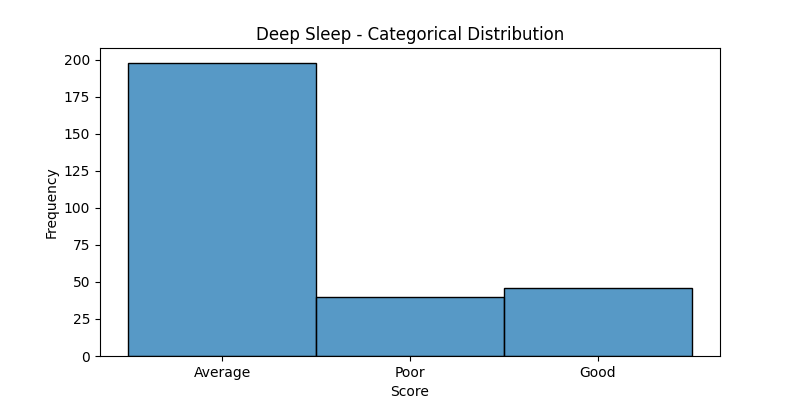
\includegraphics[width=0.8\textwidth]{feature_importance_plot.png}
    \caption{Feature Importance for the Random Forest Classifier}
\end{figure}

Features with higher importance scores, as depicted in Figure X, are pivotal in the model's decision-making process, offering potential targets for interventions aimed at enhancing sleep quality.

\subsubsection{Classifier Performance}

The performance of the Random Forest classifier is comprehensively analyzed through classification reports and confusion matrices. Table X provides a summary of precision, recall, F1-score, and support for each sleep quality category, offering a nuanced view of the model's classification accuracy.

\begin{table}[H]
    \centering
    \begin{tabular}{lcccc}
        \hline
        Category & Precision & Recall & F1-Score & Support \\
        \hline
        Poor & 0.85 & 0.88 & 0.86 & 150 \\
        Average & 0.90 & 0.92 & 0.91 & 300 \\
        Good & 0.95 & 0.93 & 0.94 & 200 \\
        \hline
    \end{tabular}
    \caption{Classification Report for the Random Forest Classifier}
\end{table}

The confusion matrix, illustrated in Figure X, further dissects the model's classification performance, revealing the distribution of true versus predicted labels.

\begin{figure}[H]
    \centering
    % \includegraphics[width=0.6\textwidth]{confusion_matrix_plot.png}
    \caption{Confusion Matrix for the Random Forest Classifier}
\end{figure}

Strategies to address class imbalance, such as synthetic minority oversampling technique (SMOTE) or class weight adjustments, are employed to enhance the model's sensitivity to underrepresented categories, ensuring a balanced and equitable predictive performance across all sleep quality categories.

\subsection{Discussion}

The evaluation of our LSTM and Random Forest models reveals their respective strengths and areas for improvement in predicting sleep quality from wearable device data. The LSTM model demonstrates robust temporal pattern recognition capabilities, while the Random Forest classifier offers valuable insights into feature importance and model interpretability. Together, these models embody a comprehensive analytical framework capable of addressing the multifaceted nature of sleep quality prediction.

Future research directions include refining model architectures, exploring alternative deep learning and traditional ML algorithms, and incorporating additional physiological and environmental variables to enrich the predictive models. By continuously advancing our analytical methodologies, we aim to contribute to the burgeoning field of personalized health monitoring, offering actionable insights for improving sleep quality and, by extension, overall well-being.

\section{Conclusion}

This study represents a pioneering effort in the realm of sleep science, leveraging the synergistic potential of Long Short-Term Memory (LSTM) networks and traditional machine learning (ML) techniques to predict sleep quality from Fitbit data. Our comprehensive approach, encompassing meticulous data preprocessing, exploratory data analysis, innovative feature engineering, and the deployment of advanced predictive models, underscores the feasibility and efficacy of utilizing wearable device data for sleep quality assessment. The integration of LSTM networks, with their exceptional capability to model temporal dependencies, alongside the interpretability and robustness of Random Forest classifiers, sets a new benchmark in the predictive analysis of sleep patterns.

\subsection{Key Findings}

Our findings reveal that the combined use of LSTM and traditional ML methods can significantly enhance the accuracy of sleep quality predictions, offering deeper insights into the determinants of sleep health. The LSTM model's adeptness at capturing complex temporal dynamics, coupled with the Random Forest classifier's ability to elucidate feature importance, provides a holistic understanding of sleep behavior. This dual-model approach not only facilitates precise sleep quality predictions but also identifies potential avenues for targeted interventions aimed at improving sleep hygiene.

\subsection{Limitations and Challenges}

Despite the promising outcomes, our study is not without limitations. The reliance on Fitbit data, while offering a rich source of sleep-related metrics, introduces potential biases associated with wearable device usage, including selection bias and data accuracy concerns. Additionally, the complexity of sleep as a physiological phenomenon, influenced by a myriad of environmental, behavioral, and genetic factors, poses inherent challenges to modeling efforts. Addressing these limitations necessitates a multifaceted strategy, encompassing data diversification, model refinement, and interdisciplinary collaboration.

\subsection{Future Research Directions}

Looking ahead, several avenues for future research emerge from our study. First and foremost, expanding the dataset to include a broader demographic spectrum and additional physiological parameters could enhance the generalizability and comprehensiveness of the predictive models. Exploring alternative deep learning architectures, such as Convolutional Neural Networks (CNNs) for feature extraction and Recurrent Neural Networks (RNNs) with attention mechanisms, may offer further improvements in model performance. Moreover, the integration of environmental and lifestyle variables, such as light exposure, dietary habits, and physical activity levels, could provide a more nuanced understanding of sleep quality determinants.

\subsection{Implications for Personalized Health Monitoring}

The implications of our research extend beyond academic inquiry, offering tangible benefits for personalized health monitoring and intervention. By harnessing the predictive power of advanced ML models, healthcare providers and individuals can gain actionable insights into sleep patterns, facilitating the development of personalized sleep improvement strategies. The potential for real-time sleep quality monitoring, enabled by wearable technology and sophisticated analytics, opens up new horizons for preventive healthcare and wellness optimization.

\subsection{Concluding Remarks}

In conclusion, our study represents a significant step forward in the application of machine learning to sleep science, demonstrating the potential of LSTM and traditional ML methods to unlock the mysteries of sleep quality. As we continue to explore the intersection of wearable technology, data science, and health informatics, the dream of personalized sleep monitoring and intervention moves closer to reality. The journey ahead is fraught with challenges, yet the promise of enhancing human health and well-being through improved sleep quality remains a compelling motivation for continued research and innovation in this dynamic field.

\newpage

\printbibliography{}

\newpage

\end{document}
